% !TeX program = pdfLaTeX
\documentclass[12pt]{article}
\usepackage{amsmath}
\usepackage{graphicx,psfrag,epsf}
\usepackage{enumerate}
\usepackage{natbib}
\usepackage{textcomp}
\usepackage[hyphens]{url} % not crucial - just used below for the URL
\usepackage{hyperref}
\providecommand{\tightlist}{%
  \setlength{\itemsep}{0pt}\setlength{\parskip}{0pt}}

%\pdfminorversion=4
% NOTE: To produce blinded version, replace "0" with "1" below.
\newcommand{\blind}{0}

% DON'T change margins - should be 1 inch all around.
\addtolength{\oddsidemargin}{-.5in}%
\addtolength{\evensidemargin}{-.5in}%
\addtolength{\textwidth}{1in}%
\addtolength{\textheight}{1.3in}%
\addtolength{\topmargin}{-.8in}%

%% load any required packages here


\usepackage{color}
\usepackage{fancyvrb}
\newcommand{\VerbBar}{|}
\newcommand{\VERB}{\Verb[commandchars=\\\{\}]}
\DefineVerbatimEnvironment{Highlighting}{Verbatim}{commandchars=\\\{\}}
% Add ',fontsize=\small' for more characters per line
\usepackage{framed}
\definecolor{shadecolor}{RGB}{248,248,248}
\newenvironment{Shaded}{\begin{snugshade}}{\end{snugshade}}
\newcommand{\AlertTok}[1]{\textcolor[rgb]{0.94,0.16,0.16}{#1}}
\newcommand{\AnnotationTok}[1]{\textcolor[rgb]{0.56,0.35,0.01}{\textbf{\textit{#1}}}}
\newcommand{\AttributeTok}[1]{\textcolor[rgb]{0.77,0.63,0.00}{#1}}
\newcommand{\BaseNTok}[1]{\textcolor[rgb]{0.00,0.00,0.81}{#1}}
\newcommand{\BuiltInTok}[1]{#1}
\newcommand{\CharTok}[1]{\textcolor[rgb]{0.31,0.60,0.02}{#1}}
\newcommand{\CommentTok}[1]{\textcolor[rgb]{0.56,0.35,0.01}{\textit{#1}}}
\newcommand{\CommentVarTok}[1]{\textcolor[rgb]{0.56,0.35,0.01}{\textbf{\textit{#1}}}}
\newcommand{\ConstantTok}[1]{\textcolor[rgb]{0.00,0.00,0.00}{#1}}
\newcommand{\ControlFlowTok}[1]{\textcolor[rgb]{0.13,0.29,0.53}{\textbf{#1}}}
\newcommand{\DataTypeTok}[1]{\textcolor[rgb]{0.13,0.29,0.53}{#1}}
\newcommand{\DecValTok}[1]{\textcolor[rgb]{0.00,0.00,0.81}{#1}}
\newcommand{\DocumentationTok}[1]{\textcolor[rgb]{0.56,0.35,0.01}{\textbf{\textit{#1}}}}
\newcommand{\ErrorTok}[1]{\textcolor[rgb]{0.64,0.00,0.00}{\textbf{#1}}}
\newcommand{\ExtensionTok}[1]{#1}
\newcommand{\FloatTok}[1]{\textcolor[rgb]{0.00,0.00,0.81}{#1}}
\newcommand{\FunctionTok}[1]{\textcolor[rgb]{0.00,0.00,0.00}{#1}}
\newcommand{\ImportTok}[1]{#1}
\newcommand{\InformationTok}[1]{\textcolor[rgb]{0.56,0.35,0.01}{\textbf{\textit{#1}}}}
\newcommand{\KeywordTok}[1]{\textcolor[rgb]{0.13,0.29,0.53}{\textbf{#1}}}
\newcommand{\NormalTok}[1]{#1}
\newcommand{\OperatorTok}[1]{\textcolor[rgb]{0.81,0.36,0.00}{\textbf{#1}}}
\newcommand{\OtherTok}[1]{\textcolor[rgb]{0.56,0.35,0.01}{#1}}
\newcommand{\PreprocessorTok}[1]{\textcolor[rgb]{0.56,0.35,0.01}{\textit{#1}}}
\newcommand{\RegionMarkerTok}[1]{#1}
\newcommand{\SpecialCharTok}[1]{\textcolor[rgb]{0.00,0.00,0.00}{#1}}
\newcommand{\SpecialStringTok}[1]{\textcolor[rgb]{0.31,0.60,0.02}{#1}}
\newcommand{\StringTok}[1]{\textcolor[rgb]{0.31,0.60,0.02}{#1}}
\newcommand{\VariableTok}[1]{\textcolor[rgb]{0.00,0.00,0.00}{#1}}
\newcommand{\VerbatimStringTok}[1]{\textcolor[rgb]{0.31,0.60,0.02}{#1}}
\newcommand{\WarningTok}[1]{\textcolor[rgb]{0.56,0.35,0.01}{\textbf{\textit{#1}}}}

% Pandoc citation processing


\begin{document}


\def\spacingset#1{\renewcommand{\baselinestretch}%
{#1}\small\normalsize} \spacingset{1}


%%%%%%%%%%%%%%%%%%%%%%%%%%%%%%%%%%%%%%%%%%%%%%%%%%%%%%%%%%%%%%%%%%%%%%%%%%%%%%

\if0\blind
{
  \title{\bf btmembers: An R package to import data on all members of
the Bundestag since 1949}

  \author{
        Philippe Joly \\
    Otto Suhr Institute of Political Science, Free University of
Berlin\\
      }
  \maketitle
} \fi

\if1\blind
{
  \bigskip
  \bigskip
  \bigskip
  \begin{center}
    {\LARGE\bf btmembers: An R package to import data on all members of
the Bundestag since 1949}
  \end{center}
  \medskip
} \fi

\bigskip
\begin{abstract}
The Bundestag distributes biographical and election data on all its
members since 1949. This data, however, is only available in XML, a
format social scientists might find difficult to work with. This paper
introduces a tool to make the Bundestag open data more accessible: the
btmembers R package. btmembers downloads the XML file on members of the
Bundestag, converts it to a data frame, and recodes some of the
variables. The generated dataset contains more than 11,000 observations
for more than 4,000 members of the Bundestag. With its tabular format,
the dataset allows users to easily examine the evolution of the
composition of the parliament with regards to gender, age, occupation,
and other characteristics. The package is a useful resource for
researchers, journalists, teachers, and the broader public.
\end{abstract}

\noindent%
{\it Keywords:} Bundestag, parliament, open data, political
representation, R
\vfill

\newpage
\spacingset{1.45} % DON'T change the spacing!

The Bundestag website provides useful
\href{https://www.bundestag.de/services/opendata/}{resources} such as
minutes of the plenary sessions, roll call votes, and data on elected
members. Information on members of the Bundestag, however, can be
difficult to extract since it is stored in an XML file. Unlike usual
rectangular datasets, XML files have a tree-like structure. They can
organize data in an arbitrary number of dimensions. This format is not
well-suited for comparative analyses. In this short paper, I would like
to introduce a tool to make the Bundestag open data accessible to a
broader public: the btmembers R package. btmembers downloads the XML
file on members of the Bundestag, converts it to a data frame, and
recodes some of the variables. The generated dataset contains more than
11,000 observations for more than 4,000 members of the Bundestag.

\hypertarget{a-look-at-the-original-data}{%
\section{A look at the original
data}\label{a-look-at-the-original-data}}

To illustrate the challenges of working with the original XML file
provided by the Bundestag, let us have a look at the data for Elisabeth
Schwarzhaupt (CDU). Schwarzhaupt was Federal Minister of Health from
1961 to 1966 and the first woman to hold a ministerial position in
Germany.

{\scriptsize

\begin{Shaded}
\begin{Highlighting}[]
\KeywordTok{\textless{}MDB\textgreater{}}
    \KeywordTok{\textless{}ID\textgreater{}}\NormalTok{11002129}\KeywordTok{\textless{}/ID\textgreater{}}
    \KeywordTok{\textless{}NAMEN\textgreater{}}
      \KeywordTok{\textless{}NAME\textgreater{}}
        \KeywordTok{\textless{}NACHNAME\textgreater{}}\NormalTok{Schwarzhaupt}\KeywordTok{\textless{}/NACHNAME\textgreater{}}
        \KeywordTok{\textless{}VORNAME\textgreater{}}\NormalTok{Elisabeth}\KeywordTok{\textless{}/VORNAME\textgreater{}}
        \KeywordTok{\textless{}ORTSZUSATZ/\textgreater{}}
        \KeywordTok{\textless{}ADEL/\textgreater{}}
        \KeywordTok{\textless{}PRAEFIX/\textgreater{}}
        \KeywordTok{\textless{}ANREDE\_TITEL\textgreater{}}\NormalTok{Dr.}\KeywordTok{\textless{}/ANREDE\_TITEL\textgreater{}}
        \KeywordTok{\textless{}AKAD\_TITEL\textgreater{}}\NormalTok{Dr.}\KeywordTok{\textless{}/AKAD\_TITEL\textgreater{}}
        \KeywordTok{\textless{}HISTORIE\_VON\textgreater{}}\NormalTok{06.10.1953}\KeywordTok{\textless{}/HISTORIE\_VON\textgreater{}}
        \KeywordTok{\textless{}HISTORIE\_BIS/\textgreater{}}
      \KeywordTok{\textless{}/NAME\textgreater{}}
    \KeywordTok{\textless{}/NAMEN\textgreater{}}
    \KeywordTok{\textless{}BIOGRAFISCHE\_ANGABEN\textgreater{}}
      \KeywordTok{\textless{}GEBURTSDATUM\textgreater{}}\NormalTok{07.01.1901}\KeywordTok{\textless{}/GEBURTSDATUM\textgreater{}}
      \KeywordTok{\textless{}GEBURTSORT\textgreater{}}\NormalTok{Frankfurt/Main}\KeywordTok{\textless{}/GEBURTSORT\textgreater{}}
      \KeywordTok{\textless{}GEBURTSLAND/\textgreater{}}
      \KeywordTok{\textless{}STERBEDATUM\textgreater{}}\NormalTok{29.10.1986}\KeywordTok{\textless{}/STERBEDATUM\textgreater{}}
      \KeywordTok{\textless{}GESCHLECHT\textgreater{}}\NormalTok{weiblich}\KeywordTok{\textless{}/GESCHLECHT\textgreater{}}
      \KeywordTok{\textless{}FAMILIENSTAND\textgreater{}}\NormalTok{keine Angaben}\KeywordTok{\textless{}/FAMILIENSTAND\textgreater{}}
      \KeywordTok{\textless{}RELIGION\textgreater{}}\NormalTok{evangelisch}\KeywordTok{\textless{}/RELIGION\textgreater{}}
      \KeywordTok{\textless{}BERUF\textgreater{}}\NormalTok{Bundesminister für Gesundheitswesen, Oberkirchenrätin i. R.}\KeywordTok{\textless{}/BERUF\textgreater{}}
      \KeywordTok{\textless{}PARTEI\_KURZ\textgreater{}}\NormalTok{CDU}\KeywordTok{\textless{}/PARTEI\_KURZ\textgreater{}}
      \KeywordTok{\textless{}VITA\_KURZ/\textgreater{}}
      \KeywordTok{\textless{}VEROEFFENTLICHUNGSPFLICHTIGES/\textgreater{}}
    \KeywordTok{\textless{}/BIOGRAFISCHE\_ANGABEN\textgreater{}}
    \KeywordTok{\textless{}WAHLPERIODEN\textgreater{}}
      \KeywordTok{\textless{}WAHLPERIODE\textgreater{}}
        \KeywordTok{\textless{}WP\textgreater{}}\NormalTok{2}\KeywordTok{\textless{}/WP\textgreater{}}
        \KeywordTok{\textless{}MDBWP\_VON\textgreater{}}\NormalTok{06.10.1953}\KeywordTok{\textless{}/MDBWP\_VON\textgreater{}}
        \KeywordTok{\textless{}MDBWP\_BIS\textgreater{}}\NormalTok{06.10.1957}\KeywordTok{\textless{}/MDBWP\_BIS\textgreater{}}
        \KeywordTok{\textless{}WKR\_NUMMER/\textgreater{}}
        \KeywordTok{\textless{}WKR\_NAME/\textgreater{}}
        \KeywordTok{\textless{}WKR\_LAND/\textgreater{}}
        \KeywordTok{\textless{}LISTE\textgreater{}}\NormalTok{HES}\KeywordTok{\textless{}/LISTE\textgreater{}}
        \KeywordTok{\textless{}MANDATSART\textgreater{}}\NormalTok{Landesliste}\KeywordTok{\textless{}/MANDATSART\textgreater{}}
        \KeywordTok{\textless{}INSTITUTIONEN\textgreater{}}
          \KeywordTok{\textless{}INSTITUTION\textgreater{}}
            \KeywordTok{\textless{}INSART\_LANG\textgreater{}}\NormalTok{Fraktion/Gruppe}\KeywordTok{\textless{}/INSART\_LANG\textgreater{}}
            \KeywordTok{\textless{}INS\_LANG\textgreater{}}\NormalTok{Fraktion der Christlich Demokratischen Union/Christlich {-} Sozialen Union}\KeywordTok{\textless{}/INS\_LANG\textgreater{}}
            \KeywordTok{\textless{}MDBINS\_VON/\textgreater{}}
            \KeywordTok{\textless{}MDBINS\_BIS/\textgreater{}}
            \KeywordTok{\textless{}FKT\_LANG/\textgreater{}}
            \KeywordTok{\textless{}FKTINS\_VON/\textgreater{}}
            \KeywordTok{\textless{}FKTINS\_BIS/\textgreater{}}
          \KeywordTok{\textless{}/INSTITUTION\textgreater{}}
        \KeywordTok{\textless{}/INSTITUTIONEN\textgreater{}}
      \KeywordTok{\textless{}/WAHLPERIODE\textgreater{}}
      \KeywordTok{\textless{}WAHLPERIODE\textgreater{}}
        \KeywordTok{\textless{}WP\textgreater{}}\NormalTok{3}\KeywordTok{\textless{}/WP\textgreater{}}
        \KeywordTok{\textless{}MDBWP\_VON\textgreater{}}\NormalTok{15.10.1957}\KeywordTok{\textless{}/MDBWP\_VON\textgreater{}}
        \KeywordTok{\textless{}MDBWP\_BIS\textgreater{}}\NormalTok{15.10.1961}\KeywordTok{\textless{}/MDBWP\_BIS\textgreater{}}
        \KeywordTok{\textless{}WKR\_NUMMER\textgreater{}}\NormalTok{138}\KeywordTok{\textless{}/WKR\_NUMMER\textgreater{}}
        \KeywordTok{\textless{}WKR\_NAME/\textgreater{}}
        \KeywordTok{\textless{}WKR\_LAND\textgreater{}}\NormalTok{HES}\KeywordTok{\textless{}/WKR\_LAND\textgreater{}}
        \KeywordTok{\textless{}LISTE/\textgreater{}}
        \KeywordTok{\textless{}MANDATSART\textgreater{}}\NormalTok{Direktwahl}\KeywordTok{\textless{}/MANDATSART\textgreater{}}
        \KeywordTok{\textless{}INSTITUTIONEN\textgreater{}}
          \KeywordTok{\textless{}INSTITUTION\textgreater{}}
            \KeywordTok{\textless{}INSART\_LANG\textgreater{}}\NormalTok{Fraktion/Gruppe}\KeywordTok{\textless{}/INSART\_LANG\textgreater{}}
            \KeywordTok{\textless{}INS\_LANG\textgreater{}}\NormalTok{Fraktion der Christlich Demokratischen Union/Christlich {-} Sozialen Union}\KeywordTok{\textless{}/INS\_LANG\textgreater{}}
            \KeywordTok{\textless{}MDBINS\_VON/\textgreater{}}
            \KeywordTok{\textless{}MDBINS\_BIS/\textgreater{}}
            \KeywordTok{\textless{}FKT\_LANG/\textgreater{}}
            \KeywordTok{\textless{}FKTINS\_VON/\textgreater{}}
            \KeywordTok{\textless{}FKTINS\_BIS/\textgreater{}}
          \KeywordTok{\textless{}/INSTITUTION\textgreater{}}
        \KeywordTok{\textless{}/INSTITUTIONEN\textgreater{}}
      \KeywordTok{\textless{}/WAHLPERIODE\textgreater{}}
      \KeywordTok{\textless{}WAHLPERIODE\textgreater{}}
        \KeywordTok{\textless{}WP\textgreater{}}\NormalTok{4}\KeywordTok{\textless{}/WP\textgreater{}}
        \KeywordTok{\textless{}MDBWP\_VON\textgreater{}}\NormalTok{17.10.1961}\KeywordTok{\textless{}/MDBWP\_VON\textgreater{}}
        \KeywordTok{\textless{}MDBWP\_BIS\textgreater{}}\NormalTok{17.10.1965}\KeywordTok{\textless{}/MDBWP\_BIS\textgreater{}}
        \KeywordTok{\textless{}WKR\_NUMMER/\textgreater{}}
        \KeywordTok{\textless{}WKR\_NAME/\textgreater{}}
        \KeywordTok{\textless{}WKR\_LAND/\textgreater{}}
        \KeywordTok{\textless{}LISTE\textgreater{}}\NormalTok{HES}\KeywordTok{\textless{}/LISTE\textgreater{}}
        \KeywordTok{\textless{}MANDATSART\textgreater{}}\NormalTok{Landesliste}\KeywordTok{\textless{}/MANDATSART\textgreater{}}
        \KeywordTok{\textless{}INSTITUTIONEN\textgreater{}}
          \KeywordTok{\textless{}INSTITUTION\textgreater{}}
            \KeywordTok{\textless{}INSART\_LANG\textgreater{}}\NormalTok{Fraktion/Gruppe}\KeywordTok{\textless{}/INSART\_LANG\textgreater{}}
            \KeywordTok{\textless{}INS\_LANG\textgreater{}}\NormalTok{Fraktion der Christlich Demokratischen Union/Christlich {-} Sozialen Union}\KeywordTok{\textless{}/INS\_LANG\textgreater{}}
            \KeywordTok{\textless{}MDBINS\_VON/\textgreater{}}
            \KeywordTok{\textless{}MDBINS\_BIS/\textgreater{}}
            \KeywordTok{\textless{}FKT\_LANG/\textgreater{}}
            \KeywordTok{\textless{}FKTINS\_VON/\textgreater{}}
            \KeywordTok{\textless{}FKTINS\_BIS/\textgreater{}}
          \KeywordTok{\textless{}/INSTITUTION\textgreater{}}
        \KeywordTok{\textless{}/INSTITUTIONEN\textgreater{}}
      \KeywordTok{\textless{}/WAHLPERIODE\textgreater{}}
      \KeywordTok{\textless{}WAHLPERIODE\textgreater{}}
        \KeywordTok{\textless{}WP\textgreater{}}\NormalTok{5}\KeywordTok{\textless{}/WP\textgreater{}}
        \KeywordTok{\textless{}MDBWP\_VON\textgreater{}}\NormalTok{19.10.1965}\KeywordTok{\textless{}/MDBWP\_VON\textgreater{}}
        \KeywordTok{\textless{}MDBWP\_BIS\textgreater{}}\NormalTok{19.10.1969}\KeywordTok{\textless{}/MDBWP\_BIS\textgreater{}}
        \KeywordTok{\textless{}WKR\_NUMMER/\textgreater{}}
        \KeywordTok{\textless{}WKR\_NAME/\textgreater{}}
        \KeywordTok{\textless{}WKR\_LAND/\textgreater{}}
        \KeywordTok{\textless{}LISTE\textgreater{}}\NormalTok{HES}\KeywordTok{\textless{}/LISTE\textgreater{}}
        \KeywordTok{\textless{}MANDATSART\textgreater{}}\NormalTok{Landesliste}\KeywordTok{\textless{}/MANDATSART\textgreater{}}
        \KeywordTok{\textless{}INSTITUTIONEN\textgreater{}}
          \KeywordTok{\textless{}INSTITUTION\textgreater{}}
            \KeywordTok{\textless{}INSART\_LANG\textgreater{}}\NormalTok{Fraktion/Gruppe}\KeywordTok{\textless{}/INSART\_LANG\textgreater{}}
            \KeywordTok{\textless{}INS\_LANG\textgreater{}}\NormalTok{Fraktion der Christlich Demokratischen Union/Christlich {-} Sozialen Union}\KeywordTok{\textless{}/INS\_LANG\textgreater{}}
            \KeywordTok{\textless{}MDBINS\_VON\textgreater{}}\NormalTok{19.10.1965}\KeywordTok{\textless{}/MDBINS\_VON\textgreater{}}
            \KeywordTok{\textless{}MDBINS\_BIS\textgreater{}}\NormalTok{19.10.1969}\KeywordTok{\textless{}/MDBINS\_BIS\textgreater{}}
            \KeywordTok{\textless{}FKT\_LANG/\textgreater{}}
            \KeywordTok{\textless{}FKTINS\_VON/\textgreater{}}
            \KeywordTok{\textless{}FKTINS\_BIS/\textgreater{}}
          \KeywordTok{\textless{}/INSTITUTION\textgreater{}}
        \KeywordTok{\textless{}/INSTITUTIONEN\textgreater{}}
      \KeywordTok{\textless{}/WAHLPERIODE\textgreater{}}
    \KeywordTok{\textless{}/WAHLPERIODEN\textgreater{}}
  \KeywordTok{\textless{}/MDB\textgreater{}}
\end{Highlighting}
\end{Shaded}

}

The file distributed by the Bundestag contains an
XML-\href{https://en.wikipedia.org/wiki/Node_(computer_science)}{node}
named \texttt{MDB} (Mitglied des Deutschen Bundestages) for each member
of the Bundestag. This node has four
\href{https://en.wikipedia.org/wiki/Tree_(data_structure)}{children}:
\texttt{ID} (id), \texttt{NAMEN} (names), \texttt{BIOGRAFISCHE\_ANGABEN}
(biographical information), and \texttt{WAHLPERIODEN} (parliamentary
terms). All of these four children, except \texttt{ID}, have
descendants, that is, data nested within different dimensions. In the
example above, we see that Elisabeth Schwarzhaupt was born on January 7,
1901 in Frankfurt and died on October 20, 1986. She served four terms
from 1953 to 1969.

Now, how do we combine information on multiple members? If we are not
only interested in a specific member of the Bundestag but want to
compare groups of members, we need a different data structure. I was
faced with this problem while working on a chapter in an edited volume
on the AfD\footnote{Schroeder, W., Weßels, B., \& and Joly, P. (2019).
  Die AfD als Provokateur: Metamorphosen einer Partei zwischen Parlament
  und Bewegung. In W. Schroeder \& B. Weßels (Eds.), \emph{Smarte
  Spalter: Die AfD zwischen Bewegung und Parlament} (pp.~221-256). Bonn:
  Dietz.} and started preparing R scripts to reshape the data. A few
months later, I turned these scripts into a proper package to hopefully
make the Bundestag open data a little more accessible. In the rest of
this paper, I will introduce the btmembers R package, its applications,
its remaining problems, and some potential improvements in the future.

\hypertarget{getting-started-with-btmembers}{%
\section{Getting started with
btmembers}\label{getting-started-with-btmembers}}

The objective of btmembers is to import the file ``Stammdaten aller
Abgeordneten seit 1949 im XML-Format'' and turn it into a tidy
rectangular dataset. This involves both the mechanical operation of
moving values into tabular cells and some choices about what information
to keep or drop. The unit of analysis in the generated dataset is a
member-term. In other words, each member can have multiple observations
(multiple rows). Some variables are constant for each member (e.g., date
of birth) while others vary over time (e.g., start date of a
parliamentary term). The dataset preserves almost all of the original
data, except two elements:

\begin{itemize}
\tightlist
\item
  Only the most recent names of the member are preserved. Members can
  have multiple names, for example if they got married (or divorced).
\item
  The ``functions'' of the member during a parliamentary term are not
  reported. Term variables are already nested in member variables.
  Incorporating the functions into the dataset would add yet another
  level of analysis since members can carry out multiple functions
  during the same term. This would make the structure of the dataset too
  complex. Furthermore, a look at the original data revealed that this
  variable was not coded systematically. It often omits functions
  carried out by the members. Information on functions is much more
  detailed for current than for previous members.
\end{itemize}

I will address some of the concerns related to the omission of these
pieces of information at the end of this paper. The next sections
describe how to import the data processed by btmembers.

\hypertarget{installation}{%
\subsection{Installation}\label{installation}}

btmembers is currently hosted on
\href{https://github.com/jolyphil/btmembers}{GitHub}. I am considering
submitting to CRAN at a later stage. For now, you can install the
package using \texttt{devtools}.

\begin{Shaded}
\begin{Highlighting}[]
\CommentTok{\# install.packages("devtools")}
\NormalTok{devtools}\SpecialCharTok{::}\FunctionTok{install\_github}\NormalTok{(}\StringTok{"jolyphil/btmembers"}\NormalTok{)}
\end{Highlighting}
\end{Shaded}

\hypertarget{preloaded-data}{%
\subsection{Preloaded data}\label{preloaded-data}}

btmembers comes preloaded with the processed tabular dataset. The data
is stored in an object called \texttt{members} and can be retrieved as
follows:\footnote{A CSV version of the dataset is also available on
  \href{https://github.com/jolyphil/btmembers/blob/master/csv/}{GitHub}
  .}

\begin{Shaded}
\begin{Highlighting}[]
\FunctionTok{library}\NormalTok{(btmembers)}
\NormalTok{members}
\end{Highlighting}
\end{Shaded}

\begin{verbatim}
## # A tibble: 11,627 x 26
##    id       nachname  vorname adel  praefix anrede_titel akad_titel geburtsdatum
##    <chr>    <chr>     <chr>   <chr> <chr>   <chr>        <chr>      <date>      
##  1 11000001 Abelein   Manfred <NA>  <NA>    Dr.          Prof. Dr.  1930-10-20  
##  2 11000001 Abelein   Manfred <NA>  <NA>    Dr.          Prof. Dr.  1930-10-20  
##  3 11000001 Abelein   Manfred <NA>  <NA>    Dr.          Prof. Dr.  1930-10-20  
##  4 11000001 Abelein   Manfred <NA>  <NA>    Dr.          Prof. Dr.  1930-10-20  
##  5 11000001 Abelein   Manfred <NA>  <NA>    Dr.          Prof. Dr.  1930-10-20  
##  6 11000001 Abelein   Manfred <NA>  <NA>    Dr.          Prof. Dr.  1930-10-20  
##  7 11000001 Abelein   Manfred <NA>  <NA>    Dr.          Prof. Dr.  1930-10-20  
##  8 11000002 Achenbach Ernst   <NA>  <NA>    Dr.          Dr.        1909-04-09  
##  9 11000002 Achenbach Ernst   <NA>  <NA>    Dr.          Dr.        1909-04-09  
## 10 11000002 Achenbach Ernst   <NA>  <NA>    Dr.          Dr.        1909-04-09  
## # ... with 11,617 more rows, and 18 more variables: geburtsort <chr>,
## #   geburtsland <chr>, sterbedatum <date>, geschlecht <chr>,
## #   familienstand <chr>, religion <chr>, beruf <chr>, partei_kurz <chr>,
## #   vita_kurz <chr>, veroeffentlichungspflichtiges <chr>, wp <int>,
## #   mdbwp_von <date>, mdbwp_bis <date>, wkr_nummer <int>, wkr_name <chr>,
## #   wkr_land <chr>, liste <chr>, mandatsart <chr>
\end{verbatim}

\hypertarget{variables}{%
\subsection{Variables}\label{variables}}

The current version of the dataset (2021-03-12) contains 11627
observations from 4089 members. The data includes 26 variables (in
German):\footnote{A codebook is available in the associated help page
  (\texttt{?members}) and on
  \href{https://github.com/jolyphil/btmembers/blob/master/codebook/codebook.pdf}{GitHub}
  .}

{\scriptsize

\begin{tabular}{l|l|l}
\hline
Variable & Type & Label\\
\hline
id & character & Identifikationsnummer\\
\hline
nachname & character & Nachname\\
\hline
vorname & character & Vorname\\
\hline
adel & character & Adelsprädikat\\
\hline
praefix & character & Namenspräfix\\
\hline
anrede\_titel & character & Anrede-Titel\\
\hline
akad\_titel & character & Akademischer Titel\\
\hline
geburtsdatum & Date & Geburtsdatum\\
\hline
geburtsort & character & Geburtsort\\
\hline
geburtsland & character & Geburtsland\\
\hline
sterbedatum & Date & Sterbedatum\\
\hline
geschlecht & character & Geschlecht\\
\hline
familienstand & character & Familienstand\\
\hline
religion & character & Religion\\
\hline
beruf & character & Beruf\\
\hline
partei\_kurz & character & Parteizugehörigkeit, kurzform\\
\hline
vita\_kurz & character & Kurzbiografie des Abgeordneten (nur aktuelle Wahlperiode)\\
\hline
veroeffentlichungspflichtiges & character & Veröffentlichungspflichtige Angaben (nur aktuelle Wahlperiode)\\
\hline
wp & integer & Nummer der Wahlperiode\\
\hline
mdbwp\_von & Date & Beginn der Wahlperiodenzugehörigkeit\\
\hline
mdbwp\_bis & Date & Ende der Wahlperiodenzugehörigkeit\\
\hline
wkr\_nummer & integer & Nummer des Wahlkreises\\
\hline
wkr\_name & character & Wahlkreisname\\
\hline
wkr\_land & character & Bundesland des Wahlkreises\\
\hline
liste & character & Liste\\
\hline
mandatsart & character & Art des Mandates\\
\hline
\end{tabular}

}

\hypertarget{updating-the-data}{%
\subsection{Updating the data}\label{updating-the-data}}

One of the main advantage of btmembers over other available datasets is
the easiness with which users can update the data. The Bundestag updates
the XML file a few times every year.

The version of the dataset preloaded with your installation of btmembers
is stored as an attribute of the \texttt{members} object. You can find
the version loaded on your machine by proceeding as follows:

\begin{Shaded}
\begin{Highlighting}[]
\FunctionTok{attr}\NormalTok{(members, }\StringTok{"version"}\NormalTok{)}
\end{Highlighting}
\end{Shaded}

\begin{verbatim}
## [1] "2021-03-12"
\end{verbatim}

To check if a more recent version of the data is available on the
bundestag website, simply call the following function:

\begin{Shaded}
\begin{Highlighting}[]
\FunctionTok{update\_available}\NormalTok{()}
\end{Highlighting}
\end{Shaded}

\begin{verbatim}
## You currently have the most recent version of the data.
\end{verbatim}

\begin{verbatim}
## [1] FALSE
\end{verbatim}

If \texttt{update\_available()} returns \texttt{TRUE}, you can import a
more recent version of the dataset using \texttt{import\_members()}.
This function will follow the same procedure that generated the
preloaded dataset. Importing and converting a new version of the dataset
might take 2 to 3 minutes.

\begin{Shaded}
\begin{Highlighting}[]
\NormalTok{members\_new }\OtherTok{\textless{}{-}} \FunctionTok{import\_members}\NormalTok{()}
\end{Highlighting}
\end{Shaded}

Note that \texttt{members\_new} is only stored in your global
environment. You may save it on your disk using \texttt{saveRDS()}.

\begin{Shaded}
\begin{Highlighting}[]
\FunctionTok{saveRDS}\NormalTok{(members\_new, }\StringTok{"members\_new.rds"}\NormalTok{)}
\end{Highlighting}
\end{Shaded}

\hypertarget{applications}{%
\section{Applications}\label{applications}}

btmembers is particularly useful for research on political
representation. It is also a great tool for teaching.

\hypertarget{research-on-political-representation}{%
\subsection{Research on political
representation}\label{research-on-political-representation}}

Descriptive representation is the idea that the composition of
parliaments (for example, in terms of gender, age, ethnicity, and social
structure) should mirror the constituencies represented by elected
members. With btmembers, it is easy to track the representation of
certain groups in the Bundestag, for example, women. Below is an example
showing how to examine the representation of women in different factions
over time.

\begin{Shaded}
\begin{Highlighting}[]
\FunctionTok{library}\NormalTok{(dplyr)}
\NormalTok{share\_women }\OtherTok{\textless{}{-}}\NormalTok{ members }\SpecialCharTok{\%\textgreater{}\%}
  \FunctionTok{mutate}\NormalTok{(}\AttributeTok{faction =} \FunctionTok{case\_when}\NormalTok{(}
\NormalTok{    partei\_kurz }\SpecialCharTok{==} \StringTok{"CDU"} \SpecialCharTok{|}\NormalTok{ partei\_kurz }\SpecialCharTok{==} \StringTok{"CSU"} \SpecialCharTok{\textasciitilde{}} \StringTok{"Union"}\NormalTok{,}
\NormalTok{    partei\_kurz }\SpecialCharTok{==} \StringTok{"SPD"} \SpecialCharTok{\textasciitilde{}} \StringTok{"SPD"}\NormalTok{,}
\NormalTok{    partei\_kurz }\SpecialCharTok{==} \StringTok{"FDP"} \SpecialCharTok{\textasciitilde{}} \StringTok{"FDP"}\NormalTok{)) }\SpecialCharTok{\%\textgreater{}\%}
  \FunctionTok{filter}\NormalTok{(}\SpecialCharTok{!}\FunctionTok{is.na}\NormalTok{(faction)) }\SpecialCharTok{\%\textgreater{}\%}
  \FunctionTok{group\_by}\NormalTok{(faction, wp) }\SpecialCharTok{\%\textgreater{}\%}
  \FunctionTok{summarize}\NormalTok{(}\AttributeTok{women =} \FunctionTok{mean}\NormalTok{(geschlecht }\SpecialCharTok{==} \StringTok{"weiblich"}\NormalTok{))}
\end{Highlighting}
\end{Shaded}

\begin{Shaded}
\begin{Highlighting}[]
\FunctionTok{library}\NormalTok{(ggplot2)}
\FunctionTok{ggplot}\NormalTok{(}\AttributeTok{data =}\NormalTok{ share\_women, }\FunctionTok{aes}\NormalTok{(}\AttributeTok{x =}\NormalTok{ wp, }\AttributeTok{y =}\NormalTok{ women, }\AttributeTok{color =}\NormalTok{ faction)) }\SpecialCharTok{+}
  \FunctionTok{geom\_point}\NormalTok{() }\SpecialCharTok{+}
  \FunctionTok{geom\_smooth}\NormalTok{() }\SpecialCharTok{+}
  \FunctionTok{scale\_x\_continuous}\NormalTok{(}\AttributeTok{expand =} \FunctionTok{c}\NormalTok{(}\DecValTok{0}\NormalTok{,}\DecValTok{0}\NormalTok{), }\AttributeTok{breaks =} \DecValTok{1}\SpecialCharTok{:}\DecValTok{19}\NormalTok{) }\SpecialCharTok{+}
  \FunctionTok{scale\_color\_manual}\NormalTok{(}\AttributeTok{values=}\FunctionTok{c}\NormalTok{(}\StringTok{"yellow"}\NormalTok{, }\StringTok{"red"}\NormalTok{, }\StringTok{"black"}\NormalTok{)) }\SpecialCharTok{+}
  \FunctionTok{ggtitle}\NormalTok{(}\StringTok{"Share of female members by faction"}\NormalTok{) }\SpecialCharTok{+}
  \FunctionTok{xlab}\NormalTok{(}\StringTok{"Parliamentary terms"}\NormalTok{) }\SpecialCharTok{+} 
  \FunctionTok{ylab}\NormalTok{(}\StringTok{"Share of female members"}\NormalTok{)}
\end{Highlighting}
\end{Shaded}

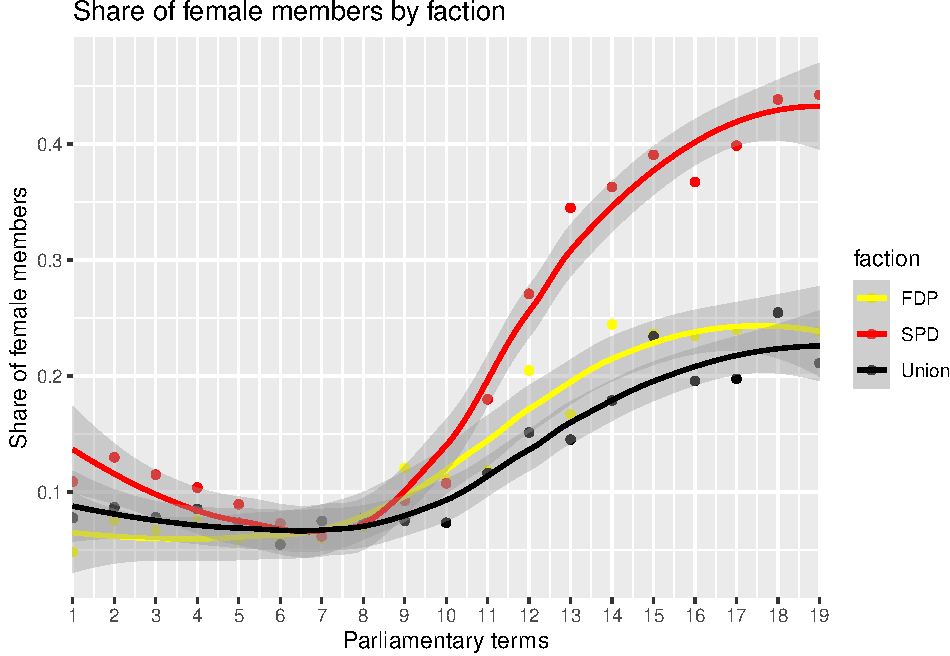
\includegraphics{paper_files/figure-latex/women_graph-1.pdf}

The figure above shows that the share of female members in the FDP, SPD,
and CDU/CSU factions remained very low---usually below 10
percent---until the end of the 1970s (8th parliamentary term). It then
grew to reach about 20\% in the FDP and CDU/CSU factions and over 40\%
in the SPD faction.

We can also have a look at changes in the occupational structure of
members over time. The code below returns the ten most common
occupations of members of the first parliamentary term (1949-09-07 to
1953-09-07).

\begin{Shaded}
\begin{Highlighting}[]
\FunctionTok{sort}\NormalTok{(}\FunctionTok{table}\NormalTok{(members}\SpecialCharTok{$}\NormalTok{beruf[members}\SpecialCharTok{$}\NormalTok{wp }\SpecialCharTok{==} \DecValTok{1}\NormalTok{]), }\AttributeTok{decreasing =}\NormalTok{ T)[}\DecValTok{1}\SpecialCharTok{:}\DecValTok{10}\NormalTok{]}
\end{Highlighting}
\end{Shaded}

\begin{verbatim}
## 
##               Landwirt           Rechtsanwalt               Kaufmann 
##                     20                     20                     15 
##           Angestellter Rechtsanwalt und Notar              Redakteur 
##                     13                     10                     10 
##   Bundesminister a. D.              Fabrikant               Hausfrau 
##                      9                      9                      8 
##             Journalist 
##                      8
\end{verbatim}

And the code below returns the ten most common occupations of members of
the current parliamentary term (since 2017-10-24).

\begin{Shaded}
\begin{Highlighting}[]
\FunctionTok{sort}\NormalTok{(}\FunctionTok{table}\NormalTok{(members}\SpecialCharTok{$}\NormalTok{beruf[members}\SpecialCharTok{$}\NormalTok{wp }\SpecialCharTok{==} \DecValTok{19}\NormalTok{]), }\AttributeTok{decreasing =}\NormalTok{ T)[}\DecValTok{1}\SpecialCharTok{:}\DecValTok{10}\NormalTok{]}
\end{Highlighting}
\end{Shaded}

\begin{verbatim}
## 
##           Rechtsanwalt         Rechtsanwältin                 Jurist 
##                     38                     14                     11 
##               Juristin Politikwissenschaftler        Geschäftsführer 
##                      9                      8                      7 
##             Volljurist           Angestellter            Unternehmer 
##                      7                      6                      6 
##    Bürgermeister a. D. 
##                      5
\end{verbatim}

We see that occupations like farmer (``Landwirt'') and housewife
(``Hausfrau'') have been replaced by new ones like political scientist
(``Politikwissenschaftler''). Jurists were and continue to be very well
represented in the Bundestag.

\hypertarget{teaching}{%
\subsection{Teaching}\label{teaching}}

btmembers can also be used by teachers. In data analysis classes, the
package is well-suited for exercises on data visualization, clustered
data, and textual analysis (especially with the \texttt{vita\_kurz}
variable, which is available for the last parliamentary term). It is
also a great resource for classes on political representation and German
politics. It provides a structured and easily accessible repertoire of
facts about German parliamentary history.

\hypertarget{moving-forward-remaining-problems-and-potential-solutions}{%
\section{Moving forward: Remaining problems and potential
solutions}\label{moving-forward-remaining-problems-and-potential-solutions}}

There are a few remaining problems with btmembers. I note here some of
these limitations and suggest improvements for future versions of the
package.

\hypertarget{speed}{%
\subsection{Speed}\label{speed}}

btmembers is slow. Running the function \texttt{import\_members()} to
update the data can take several minutes. I am currently in the process
of integrating new functions from the package \texttt{dplyr} that should
substantially increase the speed of the function.

\hypertarget{lost-data}{%
\subsection{Lost data}\label{lost-data}}

As explained previously, all the original data provided by the Bundestag
is preserved, except previous names of members and their functions in
the Bundestag. One way to keep all the data would be to give users the
option to import not one but \emph{multiple} dataframes, for example,
one dataframe for names, one for biographical data, and one for
functions. The dataframes could then be merged using the id and
parliamentary term variables as merging keys. I am planning to implement
this option in the near future.

\hypertarget{data-update}{%
\subsection{Data update}\label{data-update}}

The data that comes preloaded with btmembers is not updated
automatically. Users have the option to run \texttt{update\_available()}
in combination with \texttt{import\_members()} to get the latest version
of the data from the Bundestag website. My long-term objective is to
incorporate automatic checks on GitHub.

\hypertarget{problems-with-the-original-data}{%
\subsection{Problems with the original
data}\label{problems-with-the-original-data}}

Some problems with btmembers do not relate to the package itself, but to
the original data provided by the Bundestag. These problems are more
difficult to fix.

\begin{enumerate}
\def\labelenumi{\arabic{enumi}.}
\item
  \textbf{Some variables should have been coded as factors}. The data
  provided by the Bundestag was not intended to be condensed in a
  tabular dataset. Sometimes different values point to the same
  underlying concept. Family status, for example, has 60 different
  values: this can certainly be simplified. For the moment, I have
  refrained from recoding these variables as I am afraid I would loose
  some valuable information. Most variables have therefore been left as
  character instead of factor variables.
\item
  \textbf{The variable \texttt{partei\_kurz} does not take into account
  changes in party affiliation}. It seems like the Bundestag only refers
  to the last affiliation, but this remains unclear.
\item
  \textbf{The variable \texttt{geburtsland} is not coded
  systematically}. In the original XML file, this variable was usually
  left empty when the member was born in Germany. Yet, the problem is
  that the borders of Germany changed over the course of the twentieth
  century and this is not reflected in the data. Should members born in
  Pomerania or Sudetenland be considered born in Germany? Also, the
  coding of countries of origin should follow an internationally agreed
  standard, such as ISO-3C. Creating an alternative variable might be
  necessary.
\end{enumerate}

These limitations should be taken into consideration when using
btmembers.

\hypertarget{conclusion}{%
\section{Conclusion}\label{conclusion}}

The Bundestag is arguably the most important democratic institution in
Germany. Yet, with currently more than 700 members, examining the
composition of this representative body can be challenging. The
btmembers R package unpacks data on members of the Bundestag since 1949
and condenses it into a tabular dataset, a format better well-suited for
comparative analyses. With federal elections scheduled in a few months,
the package will help researchers, journalists, teachers, and the
broader public get a clearer picture of the German parliament.

\bibliographystyle{agsm}
\bibliography{bibliography.bib}

\end{document}
